%% This is an example first chapter.  You should put chapter/appendix that you
%% write into a separate file, and add a line \include{yourfilename} to
%% main.tex, where `yourfilename.tex' is the name of the chapter/appendix file.
%% You can process specific files by typing their names in at the 
%% \files=
%% prompt when you run the file main.tex through LaTeX.
\newcommand{\stack}[2]{\begin{array}{c}{ #1 \\ #2 }\end{array}}

\chapter{Introduction}

\section{RNA Secondary Structure Prediction}

In the nucleus of a cell, RNA is constantly being synthesized by
transcribing sections of DNA into mobile chains built from the nucleic
acids adenine, guanine, cytosine, and uracil. These RNAs serve several
functions inside of the cell, including:

\begin{description}
\item[mRNA:] `messenger RNA' which serve as blueprints for
  proteins,
\item[tRNA:] `transfer RNA' which bond to and transport amino acids
  to the ribosome to be formed into proteins,
\item[rRNA:] `ribosomal RNA' which make up ribosomes,
\item[microRNA] which bind to mRNA and modify translation or
  degradation rates, 
\item[ncRNAs] `non-coding RNAs'  which are not involved in the
  manufacturing of proteins, instead being used as tools of the cell
  for tasks including the regulation of gene expression, or
\item[others] such as snoRNAs which recognize splice sites.
\end{description} 

The last group, ncRNAs, comprises the majority of RNAs synthesized and
have mostly unknown functions. It is unlikely that they just float
around the cell uselessly, rather they are tools the cell uses to
build and run itself. It is widely believed that the function of a
strand of RNA is directly related to its structure. While DNA is
composed of two separate strands base-paired to make a double helix,
RNA is most often found as a single stranded backbone that makes base
pairs with other parts of itself. There are considered to be 3 main
levels of structure of RNA. The \emph{primary structure} is the
sequence of nucleic acids that make up the strand of RNA
i.e. `GACCUUGGGGCCCC...'. The \emph{secondary structure} is how these
bases form base pairs (see Figure \ref{fig:loopFigure}), most often of
the Watson and Crick variety (`G-C', `A-U', although sometimes 'G-U'
is possible as well). The \emph{tertiary structure} is how the
structure bends on a larger scale as the stems and loops formed by the
secondary structure interact with each other.

Primary structure can be readily observed by modern sequencing
technology, however it is the secondary structure that determines the
shape of the molecule, which is the most important when considering
interactions with other biological molecules. The full specification
of a secondary structure state includes a list of every base
pair. Finding the secondary structure of an RNA molecule is a
different task than finding the primary structure of RNA because it
samples many states in thermal equilibrium. For an individual RNA
molecule there are many valid pairings, in fact for a sequence of
length $n$ nucleotides there are $O(1.8^n)$ secondary structures
\cite{hofacker1998combinatorics}.

%[Todo: RNA is outer-planar graph, no pseudoknots]

To describe the structural ensemble, we turn to statistical
mechanics. We approximate the RNA molecule as an isolated system in
contact with a thermal reservoir that is the cell, with each secondary
structure as a state of that system. In such a system the probability
of any state $s$ is its Boltzmann factor divided by the partition
function:
\begin{equation}
P(s) = \frac{1}{Z} e^{-\beta \Delta G(s)},
\end{equation}
where $\beta = \frac{1}{RT}$, $R$ is the gas constant, $T$ is the
temperature, and
\begin{equation}
Z = \sum_{s} e^{-\beta \Delta G(s)}.
\end{equation}

Initially researchers were satisfied with presenting the MFE (minimum
free energy) state as the state the molecule assumes in nature, after
all this state is the most probable. However we will see that, perhaps
counter-intuitively, the MFE structure is not very probable (see Figure
\ref{fig:probMFE}). Looking at the whole or sample portion of
the Boltzmann distribution, are more modern approaches for predicting
the secondary structure ensemble found in nature.

\section{The Energy Model of RNA}

Computing the partition function and probabilities is impossible
without an energy model for RNA, $\Delta G(s)$. Setting the energy of
the single-stranded (no pair) state as $E = 0$, the energy model must
accurately estimate an energy for a folded secondary structure. In
practice, the free energy of a folded RNA strand is measured by
looking at the relative concentrations of unfolded to folded states at
different temperatures noting that this should be related to the ratio
of their Boltzmann factors, $e^{-\beta \Delta G}$. The population
ratios can be determined by looking at UV absorption patterns (see UV
melting section). Whatever model is developed for computing the free
energy of a structure, the predicted MFE energy for a strand should
match the results of the UV melting experiments for that strand (this
assumption is problematic because the strand might not assume the MFE
state in solution, but that problem is not resolved in this
thesis). In general, there is typically a bonus for forming pairs
($\Delta G < 0$) and a penalty for forming loops ($\Delta G > 0$).

%% historical notes and such
In early secondary structure prediction algorithms
\cite{nussinov1980fast}, energy bonuses were assigned for any pair.
The Nussinov \& Jacobson algorithm reduced to finding the legal
folding with the most base pairs. After, it was discovered
experimentally that G-C pairs are more stable than A-U pairs. Because
of this, in further iterations the energy would be determined by
counting hydrogen bonds of canonically paired bases, assigning each
-1 kcal/mol of free energy. This would mean that GC pairs are given -3
kcals/mol, AU and GU pairs are both given -2 kcals/mol. Additionally,
certain loops were given energy penalties for forming. The Zuker and
Steigler algorithm, developed for this model, minimized the free
energy \cite{zuker1981optimal}. Both this algorithm and the previous
one had elementary dynamic programming solutions. They were useful
models to use as a baseline, however, even the second iteration was
not very accurate, on average only 20.5\% of known base pairs are
correctly predicted. Later energy models would use it as a control for
the hypothesis that they increased secondary structure prediction
accuracy \cite{mathews1999expanded}. 

Indeed, much improvement was made over the hydrogen bond model by
expanding it to include what is now called the Nearest-Neighbor
model. Experiments made it clear that energy of an RNA folding is not
just linearly dependent on the bonds that are made. There are
significant interaction effects between neighboring bases and bonds,
this is called `sequence dependence', and there are polymer physics
based free energy terms that scale logarithmically with the length of
a loop (this comes from the entropy loss to make a loop). Zuker
realized the we can represent secondary structure in terms of base
pairs or in terms of loops (including base pair stacks) which are in
the Nearest-Neighbor model. We divide our structure into its loops and
compute the energy of each loop, with a separate energy model for
each.



\begin{figure}[t]
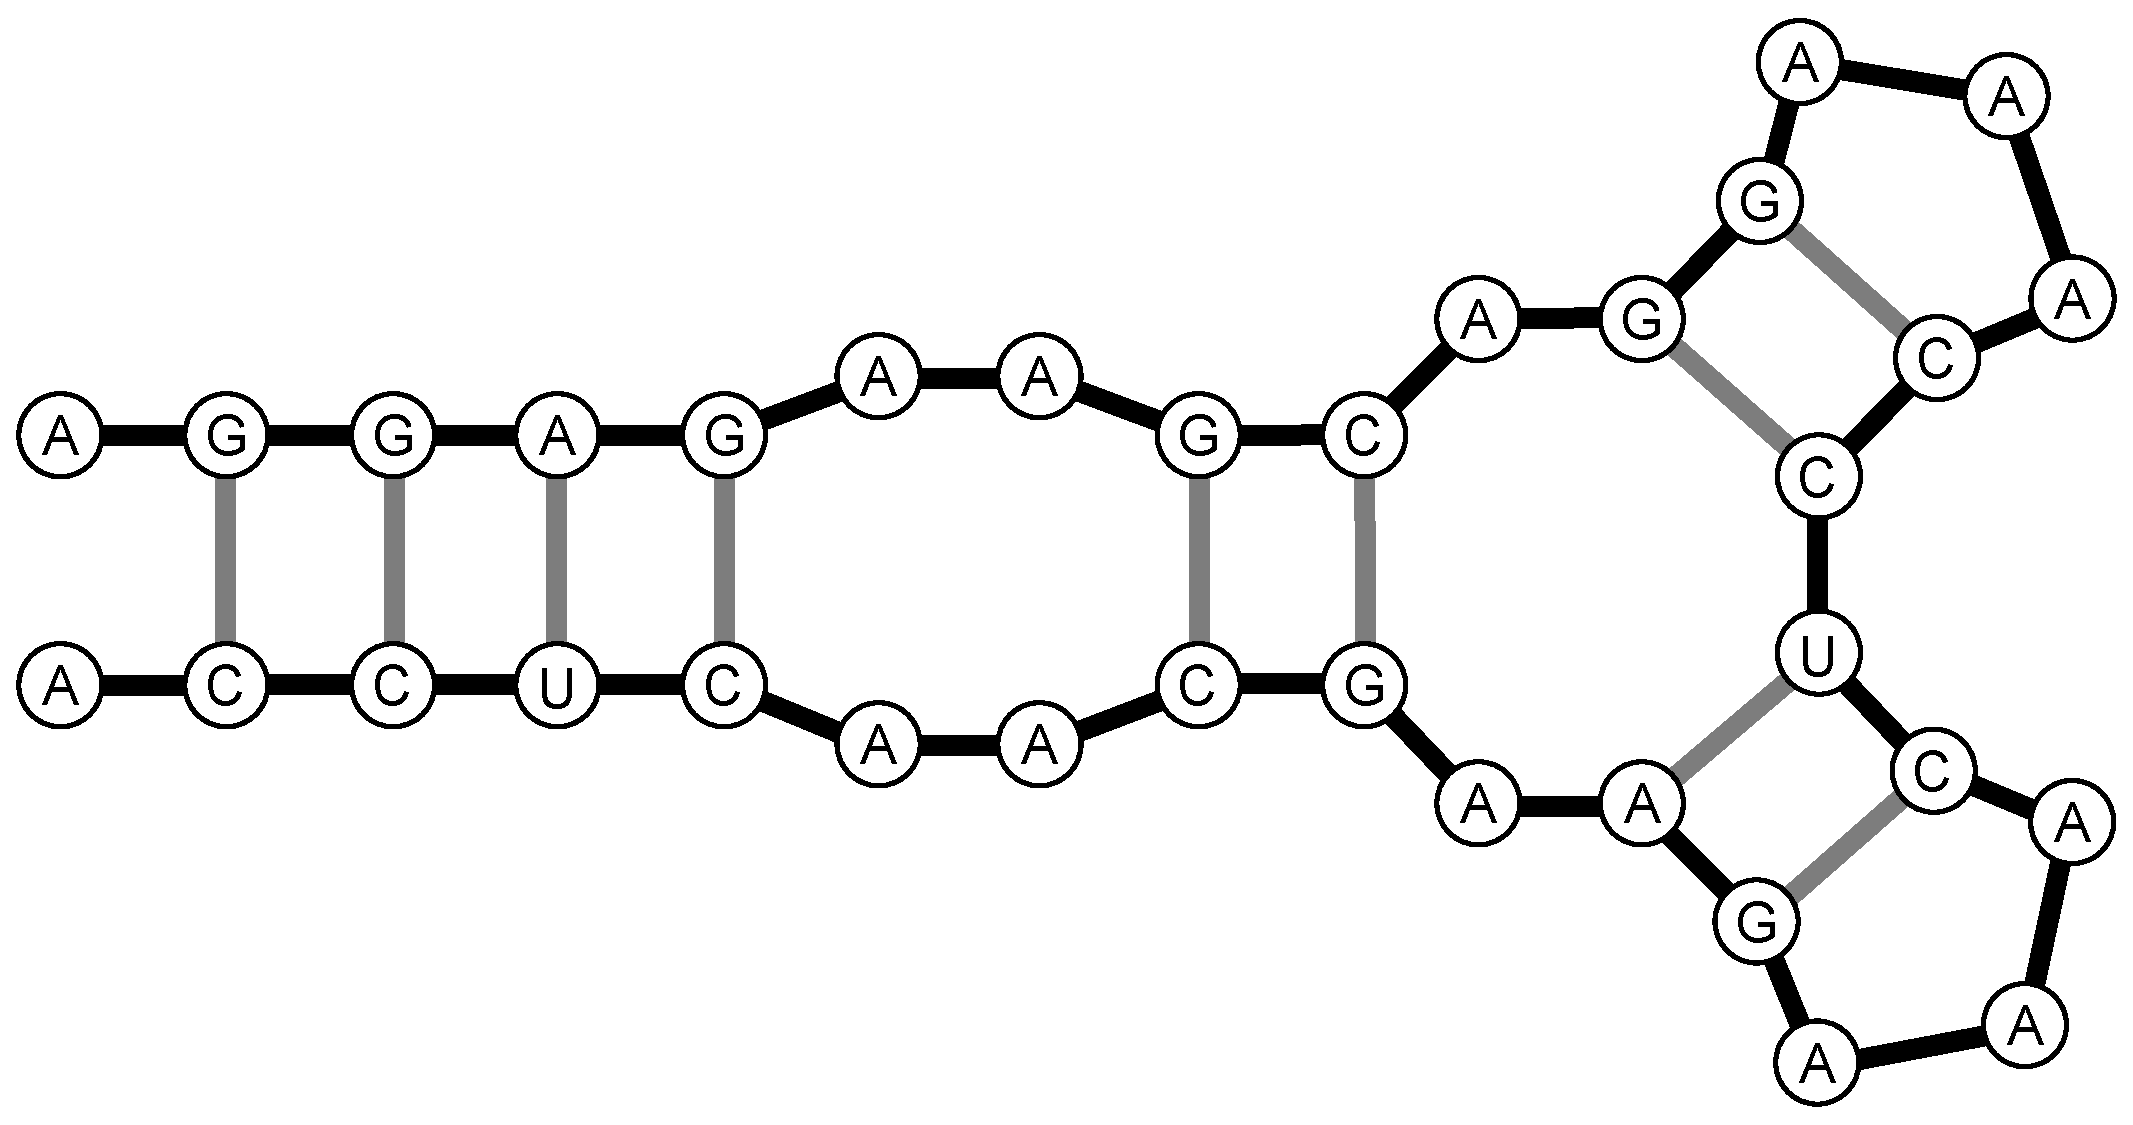
\includegraphics[width=\textwidth]{big_loop.eps}
\caption[Example Secondary Structure]{This is one possible folding out of the $O(1.8^n)$ secondary
    structures of the sequence
    `AGGAGAAGCAGGAAACCUCAAAGAACCAACUCCA'. }
\label{fig:ssExample}
\end{figure}
\begin{figure}[t]

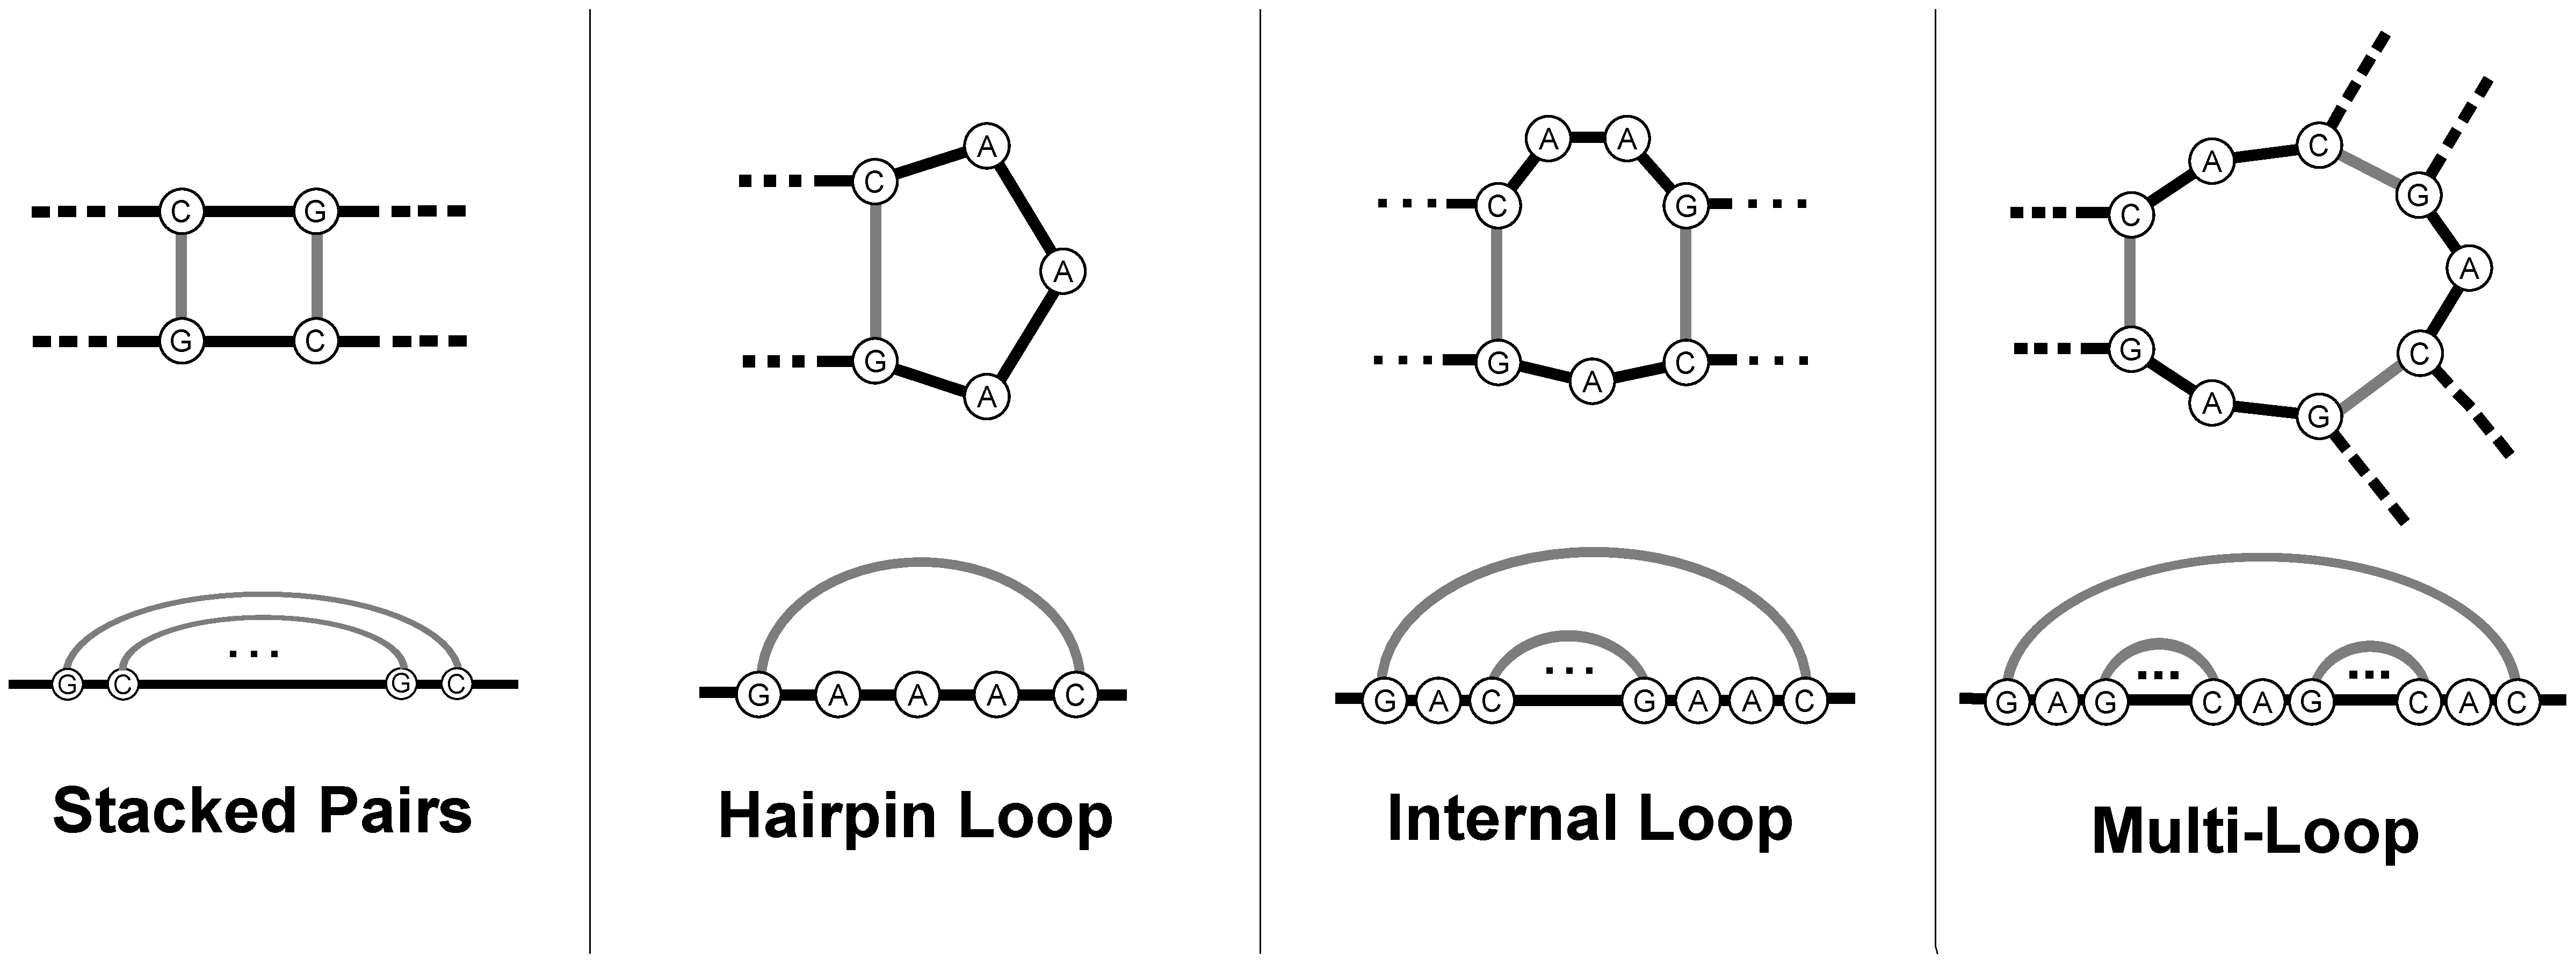
\includegraphics[width=\textwidth]{full_loop_figure.eps}
\caption[Loop Types]{The 4 types of loops, black connections are bonds in the RNA
  backbone, grey connections are hydrogen bonds between bases. The
  types are: \textit{Stacked Pairs}, adjacent pairs of bonded bases,
  \textit{Hairpin Loops}, one bonding pair closing off a turn in the
  RNA backbone, \textit{Internal Loops}, which can range from bulges
  to long loops, connecting to pairs with 2 chains of unpaired bases,
  and \textit{Multi-Loops}, which connect 3 or more pairs. The diagram
  displays the loops with how they will appear in the folded structure
  pictured above, and below is how the same loops will be laid out
  many diagrams of RNA structure, such as RNAbows
  \cite{aalberts2013visualizing}.}
\label{fig:loopFigure}
\end{figure}

In Figure \ref{fig:loopFigure}, these loops are described. In brief,
there is a different category and energy model for each type of loop
with different numbers of paired and unpaired bases. For example a
stack loop has 2 pairs and no unpaired bases. An internal loop has 2
pairs and intervening unpaired bases. A hairpin has 1 pair and any
amount of unpaired bases. Finally a multi-loop has at least 3 pairs
and unpaired bases between them.

There is a 5th type of loop, called a pseudoknot. RNA secondary
structure is normally assumed to be an outer-planar graph. A
pseudoknot consists of 2 ``crossing'' pairs. This breaks the standard
topology of the loop diagrams and makes computation of the partition
function provably NP-hard. For this reason, pseudoknots
are excluded from consideration. This is not ideal because pseudoknots
do appear in nature, notably in ribosomal RNA and at a rate of up to
12\% in Group I and Group II Introns
\cite{mathews1999expanded}. However, some of the results of this
research might make the computation of a certain restricted set of
pseduoknots much more efficient.

%[TODO: pseudoknot figure]

\subsection{Loop Parameters} 

The strand 'GGGAAACCC', will predictably form a stem-loop
structure. We can decompose the energy as such:

\begin{equation}
\Delta G \left ( \vcenter{\hbox{ 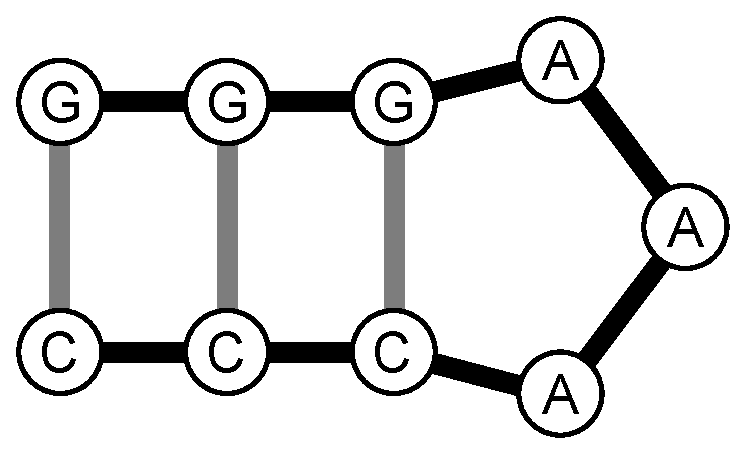
\includegraphics[scale=0.25]{stem_loop.eps}}}
 \right ) =
\Delta G_S \left ( \vcenter{\hbox{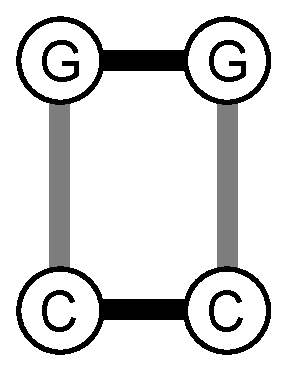
\includegraphics[scale=0.25]{GGCC-loop.eps}}}
\right ) +
\Delta G_S \left ( \vcenter{\hbox{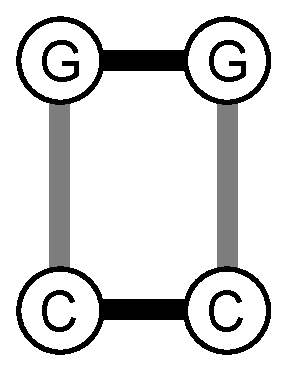
\includegraphics[scale=0.25]{GGCC-loop.eps}}}
\right ) + 
\Delta G_H \left (\vcenter{\hbox{\includegraphics[scale=0.25]{stem_loop_hairpin.eps}}}
\right )
\label{eq:decomposition}
\end{equation}

Where $\Delta G_S$ is the parameter for free energy of \emph{that
  specific} stack loop and $\Delta G_H$ is the function that gives you
the energy of a hairpin loop (which sums up the parameters of the
hairpin model).

For stack loops, the legal pairings restrict the possible loop
types. The free energy of all possible stack loops were measured, each
with a separate parameter, i.e.
\begin{equation}
\Delta G_S \left ( \vcenter{\hbox{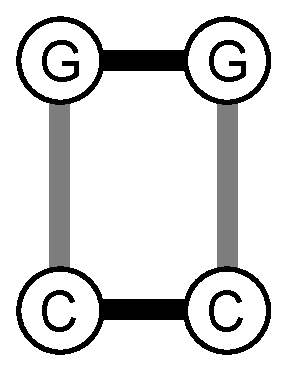
\includegraphics[scale=0.25]{GGCC-loop.eps}}}
\right ), \  
\Delta G_S \left ( \vcenter{\hbox{\includegraphics[scale=0.25]{GACU-loop.eps}}}
\right ), \ 
\Delta G_S \left ( \vcenter{\hbox{\includegraphics[scale=0.25]{AAUU-loop.eps}}}
\right ), \ \dots
\end{equation}
where each are parameters (the $\beta$s) to a linear regression model
we fit to $\Delta G$ (found from UV melting) of `GGGAAACCC' and
similar sequences.

Small internal loops and hairpins were parameterized individually but
transition to general forms for large loops to keep the model
finite. They are as follows:

\paragraph{Hairpin Loop} 
Loops with 3 and 4 unpaired bases are kept in special tables of
triloop and tetraloop parameters, respectively. Each possible
tetraloop and triloop has its own energy determined by
experiment. Beyond that, the general model is 
\begin{equation}
\begin{split}
\Delta G_H(n > 3) =  \  \Delta G_{init}(n) &+ \Delta
G_{HStack} (\text{Initializing Stack}) \\
&+ \Delta G (\text{bonuses}).
\end{split}
\end{equation}
As you can see there is an initialization term and a stack term that
are both fitted via linear regression. The bonus term is for various
special loops that have been experimentally found to be more
stable. It's outside the scope of this thesis to get into them, but
they are specified in the paper by Mathews et al \cite{mathews1999expanded}.

\paragraph{Internal Loop}
Much like stack loops, internal loops are given individual parameters
for $1 \times 1$, $1 \times 2$, $2 \times 2$, internal loops, where $n
\times m$ denotes one arm of the loop having $n$ unpaired bases and
the other having $m$. This results from extensive studies on the
$\Delta G$'s of these internal loops. For the rest of internal loops
there's a model of the form:
\begin{equation}
\begin{split}
 \Delta G_{int} ( n \times m ) = \Delta G_{init} (n + m) &+ \Delta G_{asymmetry} (| n - m |) \\
& + \Delta G ( \text{bonuses}),
\end{split}
\end{equation}
where each term on the right is a regression parameter and the bonus
term is similar to the hairpin bonus term for loops composed and ended
with certain special kinds of bases determined experimentally to be
more stable.

\paragraph{Multi-Loops}
Multi-Loops are harder to create experimental strands for and because
of this there are no individual parameters for multi loops. In fact,
for modeling multi-loops we regress to a more simple linear model of
the form:
\begin{equation}
\Delta G_{multi} = a_1 + b_1 n + c_1 h + \Delta G_{dangle},
\end{equation}
where $a_1$ is a penalty for starting a multi-loop, $n$ is the number
of unpaired bases in the loop, $b_1$ is an energy penalty per unpaired
base, $h$ is the number of pairs in the structure, $c_1$ is the energy
bonus per pair, and $\Delta G_{dangle}$ is a term similar to stack
loop terms which include the energy of the unit composed of a pair and
its 2 adjacent unpaired bases, if it has them.

%[TODO: coaxial stacking?]

\subsection{UV Melting experiments}

\begin{figure}[h]
\centering
\includegraphics{MeltingGraph.eps}

\caption[UV Melting Output]{An example of the output of a UV melting experiment. We
  should expect to see 2 levels of extinction in the graph, one
  corresponding to where single-strandedness is the equilibrium
  condition of the strand and the other where double strandedness is
  the equilibrium. As the temperature increases, the strand absorbs
  more energy from the environment allowing it to escape the
  double-stranded state and so there is a transition interval where as
  the temperature increases the UV extinction goes from the
  double-stranded extinction to the single stranded extinction.}
\label{fig:UVMeltGraph}
\end{figure}

At previously stated, loop regions are given energies as parameters to
linear regression models of free energy change in predictably folding
strands. For example, the strand `GGGAAACCC' folds predictably into a
structure with all the G's paired to the C's and a 3-A hairpin turn
(because G's pair very strongly to C's and neither are complementary
to A) as seen in Equation \ref{eq:decomposition}. David Turner
executed the following experimental process in the 90s: large amounts
of identical strands are synthesized and put into solution and
heated. A two-state assumption is made, either the RNA is folded in a
`double-stranded' state or unfolded in a `single-stranded' state. As
the solution heats, the strands will assume the unfolded, no-bonds
state. RNA is an organic, aromatic molecule that absorbs light in the
UV spectrum in different amounts depending on whether it is in a
folded state or unfolded state, so the UV absorption is fit to a curve
that then tells us about the relative concentrations of the
single-stranded vs. double-stranded state, which in turn tells us
about the free energy change between the two at a given
temperature. This free energy change is extracted and treated as a
function of the loop variables, which are then fitted to a linear
model over experiments on many different such strands
\cite{xia1998thermodynamic}.

For example, if we wanted to compute the free energy change of a
strand and fit it to its loop parameters:
\begin{equation}
\Delta G \left ( \vcenter{\hbox{ 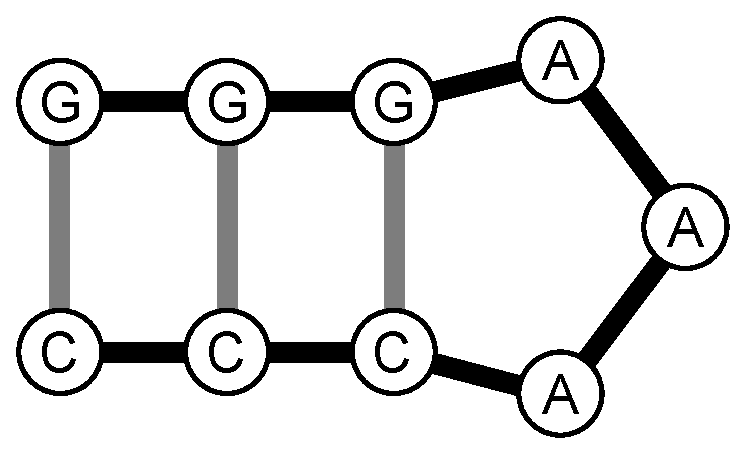
\includegraphics[scale=0.25]{stem_loop.eps}}}
 \right ) =
\Delta G_S \left ( \vcenter{\hbox{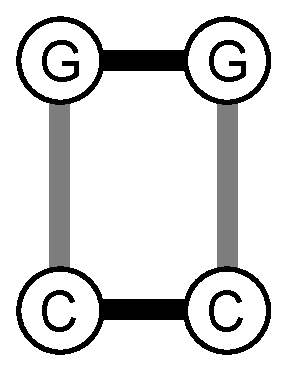
\includegraphics[scale=0.25]{GGCC-loop.eps}}}
\right ) +
\Delta G_S \left ( \vcenter{\hbox{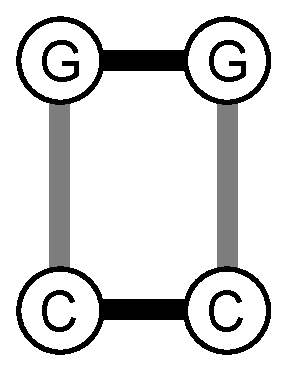
\includegraphics[scale=0.25]{GGCC-loop.eps}}}
\right ) + 
\Delta G_H \left (\vcenter{\hbox{\includegraphics[scale=0.25]{GACA-hairpin.eps}}}
\right ),
\end{equation}
we wouldq synthesize large amounts of the strand 'GGGAAACCC', put them
in solution and heat them and record their UV extinction. Observing
the curve to be like something in Figure \ref{fig:UVMeltGraph}. The
melting temperature $T_m$ is defined to be where the concentrations of
single stranded and double stranded molecules are equal, and this is
taken to be the inflection point of the graph in Figure
\ref{fig:UVMeltGraph}. From there Van't Hoff analysis is performed,
where the concentration, $C_T$, is varied and this follows a model of
the form:
\begin{equation}
  \frac{1}{T_m} = \frac{R}{\Delta H} \log{C_T} + \frac{\Delta S}{\Delta H}.
\end{equation}
This equation comes from the relation $\Delta G = -RT \log{K_{eq}}$
and plotting $1/T_m$ against $\log{C_T}$ and fitting a linear model
gives us the parameters $\Delta S$ and $\Delta H$ from the slope and
intercept and therefore $\Delta G$ through the relation
\begin{equation}
\Delta G = \Delta H - T \Delta S.
\end{equation}
Repeating this process over several strands, Turner fit the $\Delta
G$'s to a linear model based on the many parameters described in the
Loop Parameters section. From there, when we want to compute the
energy of a folding, all we have to do is separate it into loops and
sum the energies of each based off the parameters of Turner's model.


%Without the use of cool graphics, we might notate the above as:
%
%\begin{equation}
%\Delta G (GGGAAACCC) = \Delta G_s \left ( \begin{array}{c} 3' C C 5 ' \\ 5' G G 3 ' \end{array} \right ) +
%\Delta G_S \left ( \begin{array}{c} 3' C C 5 ' \\ 5' G G 3 ' \end{array} \right ) +
%\Delta G_H (G AAA C)
%\end{equation}
%
%Where $\Delta G_S $ is an individual parameter for the stack loop
%energy term and $\Delta G_H$ contains the terms for the hairpin energy
%term.

\subsection{Example Energy Computation}

Here's an example of the energy computation of a secondary structure,
pictured in Figure \ref{fig:ssExample}. There are 3 stack loop of the type:
\begin{equation}
  \Delta G \left ( \vcenter{\hbox{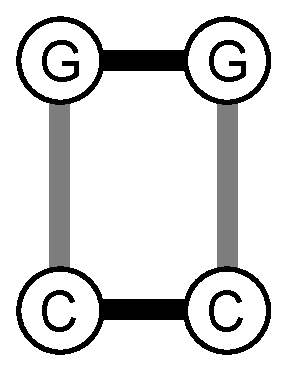
\includegraphics[scale=0.25]{GGCC-loop.eps}}}
  \right ) = -3.26 \text{ kcal/mol},
\end{equation}
and one of each:
\begin{align}
  &\Delta G \left ( \vcenter{\hbox{\includegraphics[scale=0.25]{GACU-loop.eps}}}
  \right ) = -2.35 \text{ kcal/mol},\\ 
  &\Delta G \left ( \vcenter{\hbox{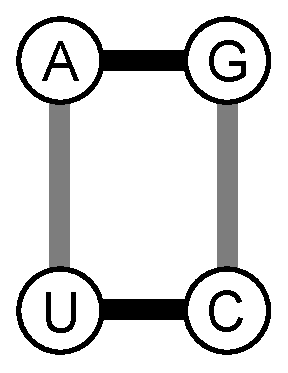
\includegraphics[scale=0.25]{AGUC-loop.eps}}}
  \right ) = -2.35 \text{ kcal/mol},\\
  &\Delta G \left ( \vcenter{\hbox{\includegraphics[scale=0.25]{UCAG-loop.eps}}}
  \right ) = -2.08 \text{ kcal/mol}.
\end{align}
These are all lookups from linear regression parameters. Besides the
stacks, there are 2 identical hairpins, an internal loop, an external
loop, and a multi-loop. For the hairpins the energy can be looked up
in a special parameter table designed specifically for hairpins with 3
unpaired bases called triloops:
\begin{align}
  \Delta G \left ( \vcenter{\hbox{\includegraphics[scale=0.25]{GACA-hairpin.eps}}}
  \right ) &= 5.8 \text{ kcal/mol}.
\end{align}
For the internal loop, there is a direct lookup for the $2 \times 2$
mismatch in a table:
\begin{align}
  \Delta G \left ( \vcenter{\hbox{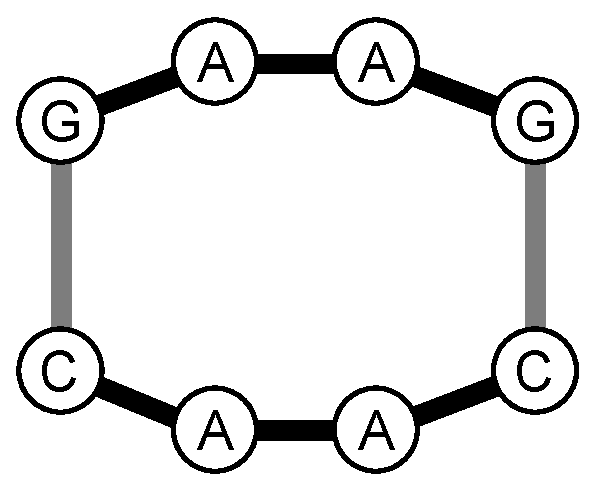
\includegraphics[scale=0.25]{GAAG-CAAC-internal-loop.eps}}}
  \right ) = 0.5 \text{ kcal/mol}.
\end{align}
The multibranch loop has 3 pairs and 2 unpaired bases. The energy is therefore:
\begin{align}
  \Delta G \left (\vcenter{\hbox{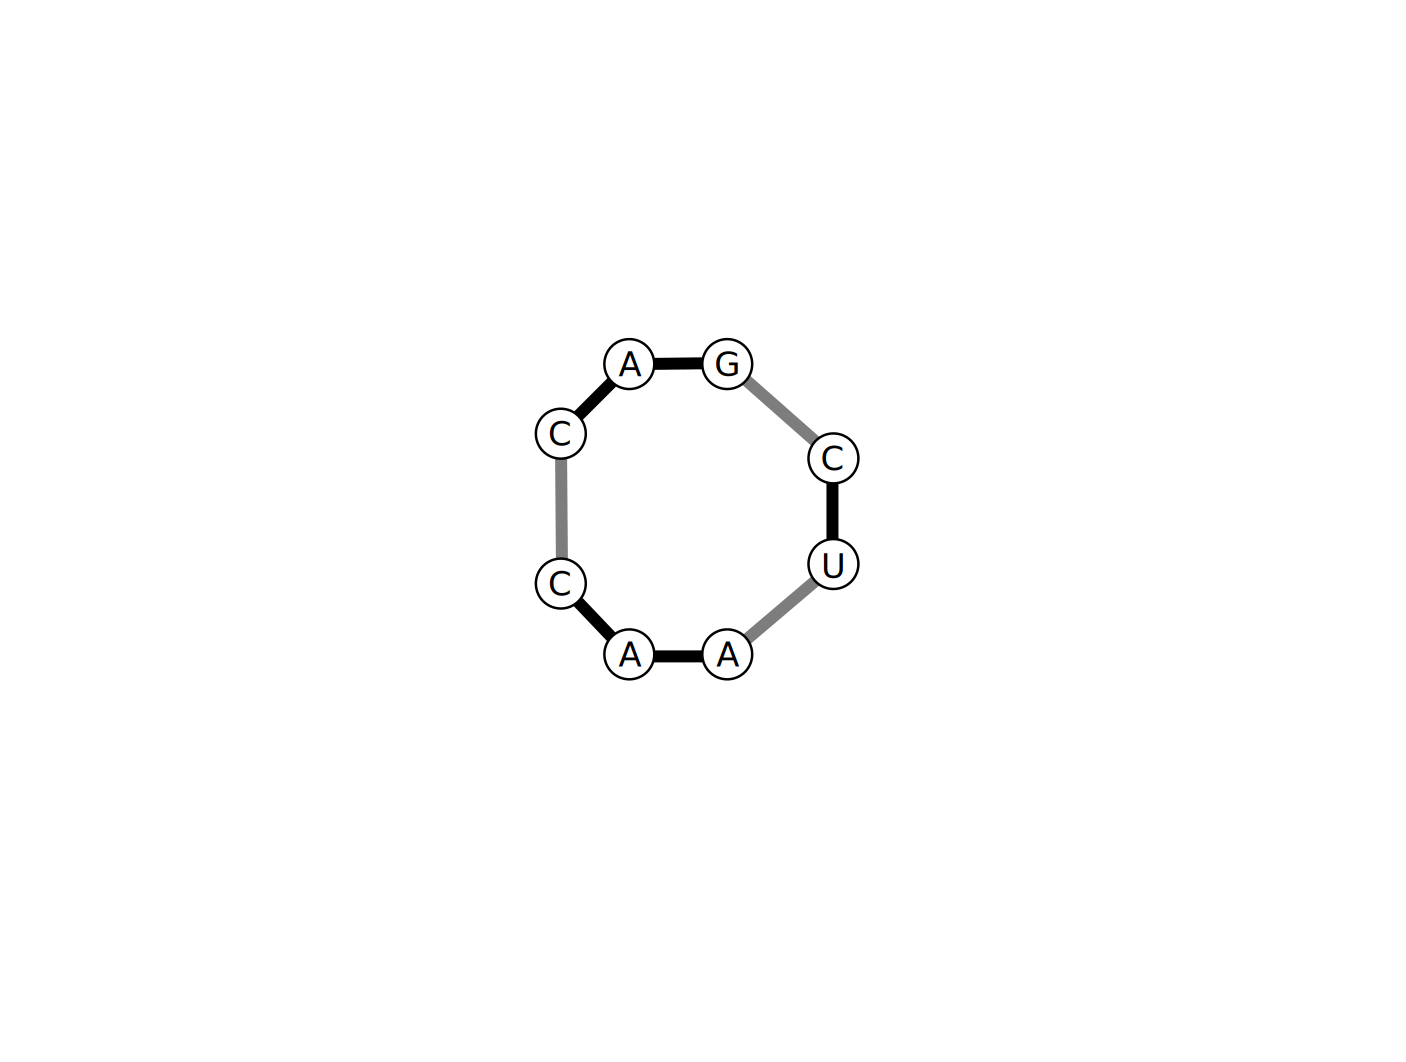
\includegraphics[scale=0.25]{CAGCUAAC-multiloop.eps}}}
  \right ) = 3.4 + 0*3 + 0.4*2 = 4.2 \text{ kcal/mol}.
\end{align}
If we sum up the contributions, we get that $\Delta G = -6.36 \text{
  kcal/mol}$. 
\section{Critique of the Energy Model}

The free energy model of RNA is not perfect. It ignores how tertiary
structure could influence the structure's stability. It is complex,
there are linear models, non-linear models, lookup tables, and
bonuses. Complexity is a very undesirable quality for a model, it
makes it hard to implement and hard for new researchers to get started
in the field.  Not only that, but many parameters have very high
error. For example, the initialization penalty for hairpin loops is
supposed to be different for different hairpin lengths, but most of
the terms aren't even $1\sigma$ away from each other. Because of this,
it is not clear what advantage these extra parameters give, perhaps
they could be reduced to one, to simplify the model greatly. Another
problem is that the data of the original experiments has been lost, so
no one can take a closer look at how well the parameters fit, and no
one seems to be interested in running the experiments
again. Additionally, the terms are heavily dependent on the salt
concentration of the solution, and great care has to be made to
imitate the conditions of the cell. It is hard to know whether the
solutions from the UV melting experiment were prepared correctly.

For these reasons, secondary structure predictions are inherently
inaccurate. However, all is not lost. Macrostate predictions collect
similar states together and this seems to average out some of the
errors associated with the model. Small disruptions, such as adding a
mutation along the strand, certainly change the $\Delta G$ of the
strand, but mutate-and-map experiments have shown that the overall
secondary structure stays relatively stable
\cite{kladwang2011two}. Therefore the error in the free energy model
provides additional motivation for the macrostate approach. 


